\begin{ledgroupsized}[r]{120mm}
\footnotesize 
\pstart  
\noindent\textbf{\"{U}berlieferung:}  
\pend
\end{ledgroupsized}
%
\begin{ledgroupsized}[r]{114mm}
\footnotesize 
\pstart
\parindent -6mm
\makebox[6mm][l]{\textit{L}}Aufzeichnung: LH XXXVII 4 Bl. 49-50. 1 Bog. 2\textsuperscript{o}. 1\,\nicefrac{1}{3} S. auf Bl. 49. Bl. 50~r\textsuperscript{o} ist leer. Bl.~50~v\textsuperscript{o} überliefert die Stücke % 037,04_49-50 = Cc2, Nr. 973
N.~43 und N.~88. Ein Wasserzeichen
% 037,04_49-50 = Cc2, Nr. 00 [Mittel, einen warmen Wind ...]
auf Bl.~49.%
% Am Rand dieses Blattes notierte Zahlenwerte: $2\frac{1}{2}, \frac{2}{2}, 2.$
\\
Cc 2, Nr. 972
\pend
\end{ledgroupsized}
%
\vspace*{5mm}
%
\begin{ledgroup}
\footnotesize
\pstart
\noindent\footnotesize{\textbf{Datierungsgr\"{u}nde}: Das vorliegende Stück handelt vom Gleichgewicht eines Balkens, bei dem Stütz- und Mittelpunkt nicht zusammenfallen. Damit besteht eine inhaltliche Verbindung mit den Stücken, die mit der Bruchfestigkeit von Balken befasst sind (siehe N.~19 bis N.~26).
 % F/1-F/8 = 037,05_201, 037,05_204, 037,05_202-203, 037,05_209, 037,05_210, 037,05_211, 037,05_207-208, 037,04_051-052
Bei nahezu all diesen Stücken ist auch das gleiche Wasserzeichen anzutreffen wie auf Bl. 49. Ihre Datierung wird demgemäß auch für das vorliegende Stück übernommen.}
\pend
\end{ledgroup}
%
\vspace{8mm}% PR: Rein provisorisch !!!
\pstart
\noindent
[49~r\textsuperscript{o}]
\pend
\vspace{0.5em}
\pstart 
%\begin{wrapfigure}{l}{0.5\textwidth}
\centering
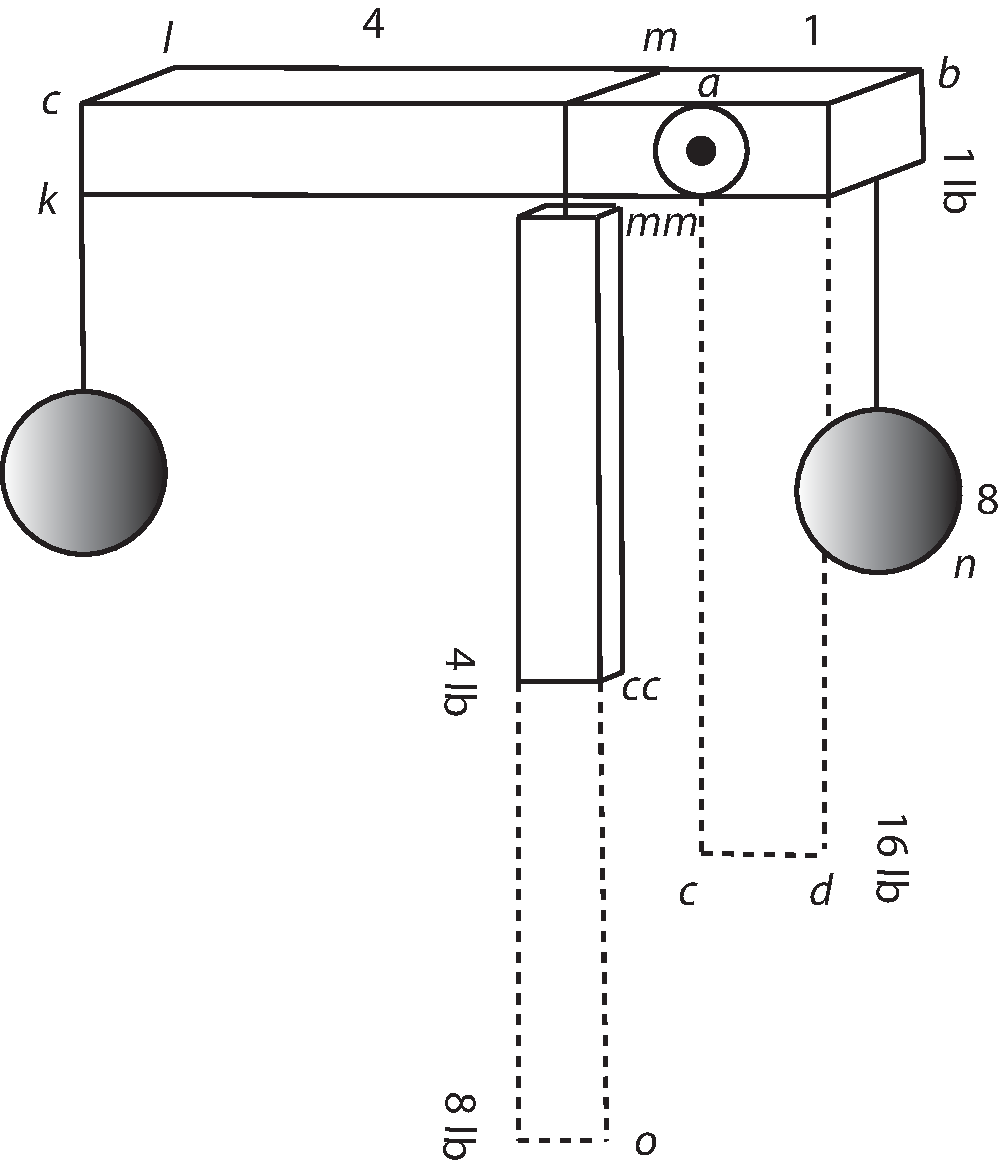
\includegraphics[width=0.58\textwidth]{images/LH37,4_49r-1.pdf}
\pend
\pstart
\vspace{2mm}
\centering
[\textit{Fig. 1}]%
%\end{wrapfigure}
\pend
\newpage%
\count\Afootins=1200
\count\Bfootins=1200
\count\Cfootins=1200
\pstart%
\normalsize%
\noindent%
Si Trabs $cab$ suspensa sit ex centro $a$ brachiis inaequalibus $ab$ et $ac$ (ita ut $ac$ sit quadrupla $ab$) quaeritur quantum ponderis\protect\index{Sachverzeichnis}{pondus} \edtext{$n$}{\lemma{$n$}\Bfootnote{\textit{erg. L}}} suspendendum sit ex $b$ ut brachium $ab$ aequilibret brachio $ac$.%
\newline%
\hspace*{7,5mm}%
Ante omnia manifestum ex mechanicis esse suppono, gravitationem\protect\index{Sachverzeichnis}{gravitatio} \edtext{seu potentiam}{\lemma{seu potentiam}\Bfootnote{\textit{erg. L}}} brachii $ac$ ad gravitationem\protect\index{Sachverzeichnis}{gravitatio} brachii $ab$ esse ut quadratum de $ac$ ad quadratum de $ab$ seu posito $ac$ ut 4 et $ab$ ut 1 esse ut 16 ad 1 et proinde si $ac$ sit quadruplo longius, $ab$ debere esse sedecuplo spissius ut $abcd$.
\pend 
\pstart%
Ratio est quod \edtext{gravitationes\protect\index{Sachverzeichnis}{gravitatio} in quolibet puncto sunt}{\lemma{gravitationes}\Bfootnote{%
\textit{(1)}\ crescunt %
\textit{(2)}\ in quolibet puncto sunt \textit{L}}} in ratione distantiarum a centro ac proinde \setline{6}exprimi possunt lineis in Triangulo $efg$ basi parallelis.
\pend
\vspace{3em}
\pstart
\hspace{-8mm}
\begin{minipage}[t]{0.5\textwidth}
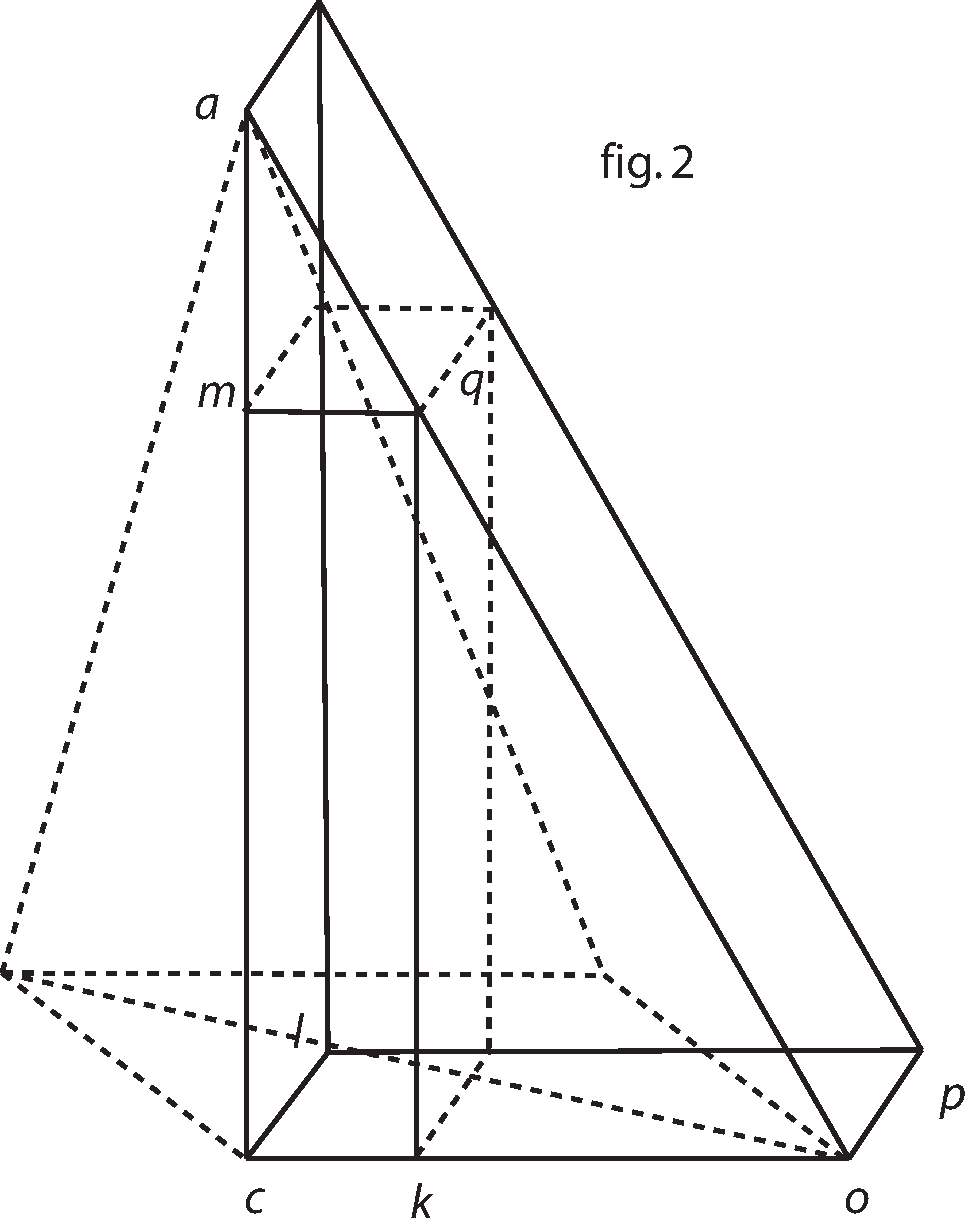
\includegraphics[width=0.95\textwidth]{images/LH37,4_49r-3.pdf}
\end{minipage}
\hspace{30mm}
\begin{minipage}[t]{0.5\textwidth}
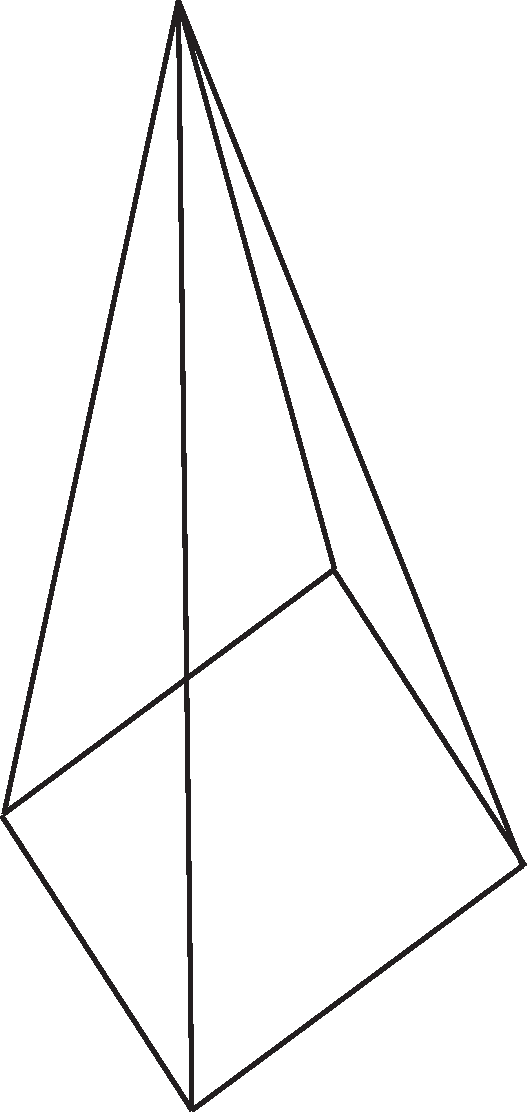
\includegraphics[width=0.45\textwidth]{images/LH37,4_49r-4.pdf}
\end{minipage}
\pend
\vspace{3mm}
\pstart
\hspace{18mm}  [\textit{Fig. 2}]\hspace*{69mm}  [\textit{Fig. 3}]
\pend
\count\Afootins=1000
\count\Bfootins=1200
\count\Cfootins=1200
\newpage
\pstart%
\begin{wrapfigure}[20]{l}{0.24\textwidth}\vspace{-5mm}
\noindent 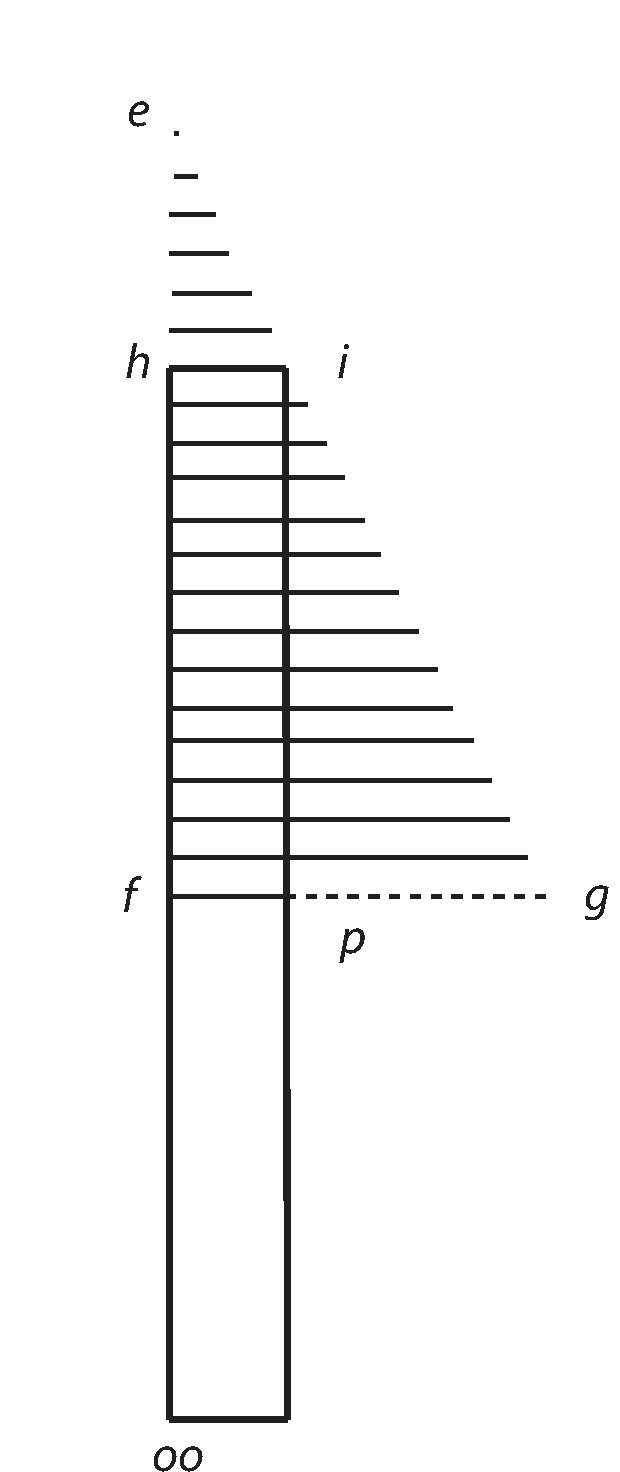
\includegraphics[trim = 19mm -1mm -5mm 17mm, clip, width=0.24\textwidth]{images/LH37,4_49r-2.pdf}\\
\noindent \centering [\textit{Fig. 4}] 
\end{wrapfigure}
Quodsi ergo in Triangulo $efg$ altitudo $ef$ sit aequalis \edtext{longitudini brachii}{\lemma{longitudini}\Bfootnote{\textit{(1)}\ vectis $a$ \textit{(2)}\ brachii \textit{L}}}\protect\index{Sachverzeichnis}{vectis} $ac$ et $eh$ aequalis $ab$ 
\edtext{et $hi$ aequalis crassitiei seu diametro trabis, nempe $ck$}{\lemma{et $hi$ [...] nempe $ck$}\Bfootnote{\textit{erg. L}}} erit ut Triang. $ehi$ ad Triang. $efg$ ita gravitatio\protect\index{Sachverzeichnis}{gravitatio} $ab$ ad gravitationem $ac$.%
%%%%%%%%%%
\edtext{}{\lemma{}\Afootnote{\textit{Nebenrechnung am Rand:}
\newline%
$ab$ vel $am$. 4.\\ 
$ac$. 12.\\
$cm$. ($ac$ - $am$). [8].\textsuperscript{[a]}\textsuperscript{[b]}\\
$ck$. latitudo trabis 3.\\ 
$cl$. crassitudo trabis 2. 
pondus\protect\index{Sachverzeichnis}{pondus} $ab$. 1 \Pfund\ ut et ei aequale $am$. Pondus $mc$. 3 \Pfund.\\
Area trabis $mlck$ est $8\smallfrown3=24\smallfrown2=48$\\
Fiat in fig. 2 ut $am$ 4. ad $ck$ 3. ita $ac$ 12 ad $co$ 9 - $ck$ 3 = $6\smallfrown$ $cl$ 2 = $ckl$ $12\smallfrown$ $mc$ 8. 96 = 48. Area prismatis\protect\index{Sachverzeichnis}{prisma} Triangularis $kopq$ vel fiat ut $am$ 4 ad $cl$ 2 ita $ac$ 12 ad $co$ 6 - $cl$ 2 = $ko$ $4\smallfrown$ $ck$ 3 = $ckl$ $12\smallfrown8$. $96\smallsmile2=48$. etc.%
% PR: Marginalienapparat:
\vspace*{2mm}% 
\newline%
\footnotesize%
\textsuperscript{[a]} 9 \textit{L \"{a}ndert Hrsg.}%
\quad%
\textsuperscript{[b]} [8]: Der Fehler wirkt sich auf die gesamte Rechnung aus und wird im Folgenden stillschweigend korrigiert.\vspace{-6mm}
}}%
%%%%%%%%%%%
\newline%
\hspace*{7.5mm}%
His positis
%ad gravitationem $ac$.%
%\edtext{}{\lemma{}\Afootnote{\textit{Nebenrechnung am Rand:}
%\newline%
%$ab$ vel $am$. 4.\\ 
%$ac$. 12. \\
%$cm$. ($ac$ - $am$). \edtext{[8].}{\Bfootnote{9 \textit{L \"{a}ndert Hrsg.}}}\edtext{}{\lemma{[8]}\Cfootnote{Der Fehler wirkt sich auf die gesamte Rechnung aus und wird im Folgenden stillschweigend korrigiert.}}\\
%$ck$. latitudo trabis 3.\\ 
%$cl$. crassitudo trabis 2. 
%pondus\protect\index{Sachverzeichnis}{pondus} $ab$. 1 \Pfund\ ut et ei aequale $am$. Pondus $mc$. 3 \Pfund.\\
%Area trabis $mlck$ est $8\smallfrown3=24\smallfrown2=48$\\
%Fiat in fig. 2 ut $am$ 4. ad $ck$ 3. ita $ac$ 12 ad $co$ 9 - $ck$ 3 = $6\smallfrown$ $cl$ 2 = $ckl$ $12\smallfrown$ $mc$ 8. 96 = 48. Area prismatis\protect\index{Sachverzeichnis}{prisma} Triangularis $kopq$ vel fiat ut $am$ 4 ad $cl$ 2 ita $ac$ 12 ad $co$ 6 - $cl$ 2 = $ko$ $4\smallfrown$ $ck$ 3 = $ckl$ $12\smallfrown8$. $96\smallsmile2=48$. etc.\vspace{-8mm}}}\\
%%\pend
%%\newpage%
%%\pstart 
%%\begin{minipage}[t]{0.4\textwidth}
%%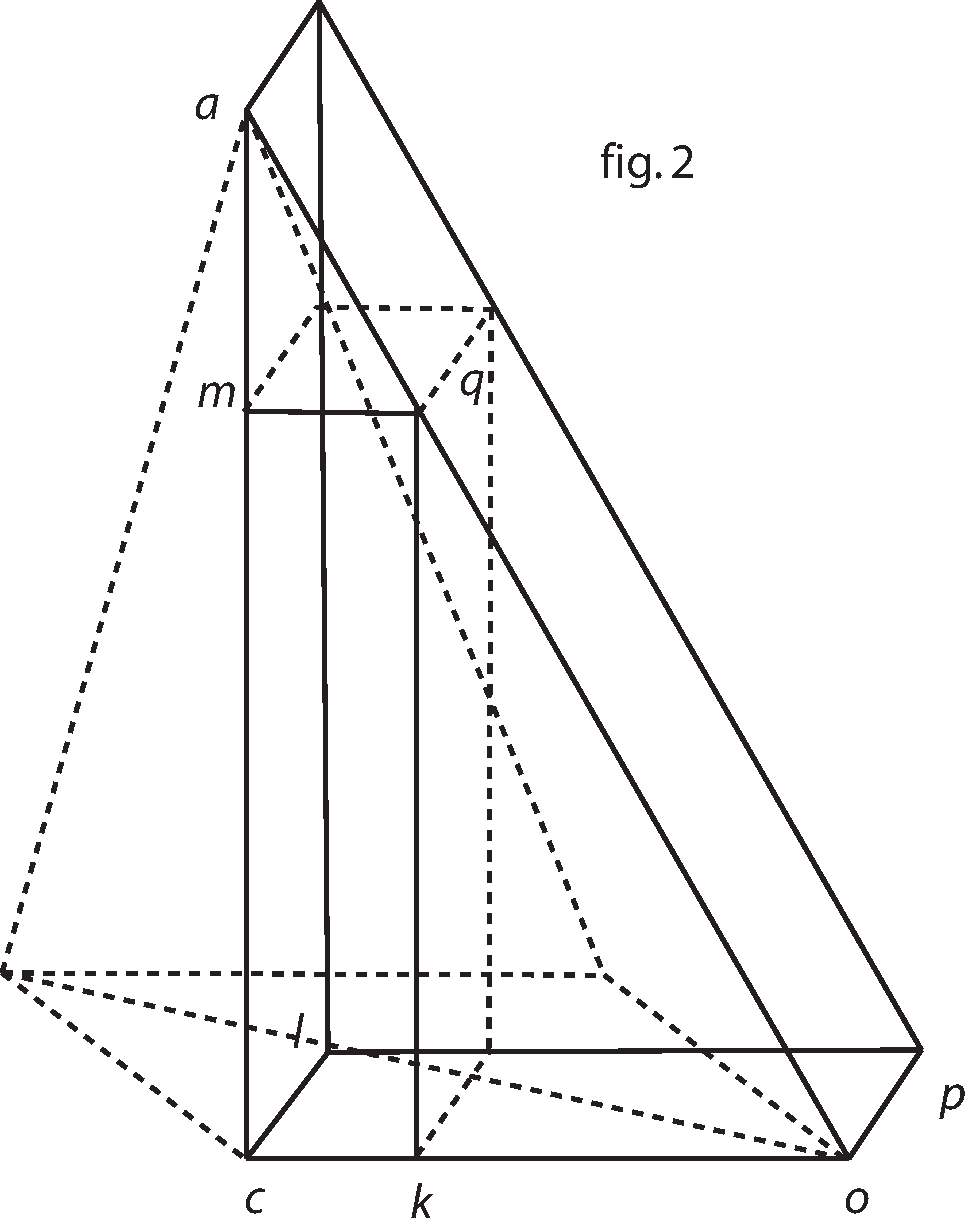
\includegraphics[width=0.6\textwidth]{images/LH37,4_49r-3.pdf}
%%\end{minipage}
%%\hspace*{13,3mm}
%%\begin{minipage}[t]{0.33\textwidth}
%%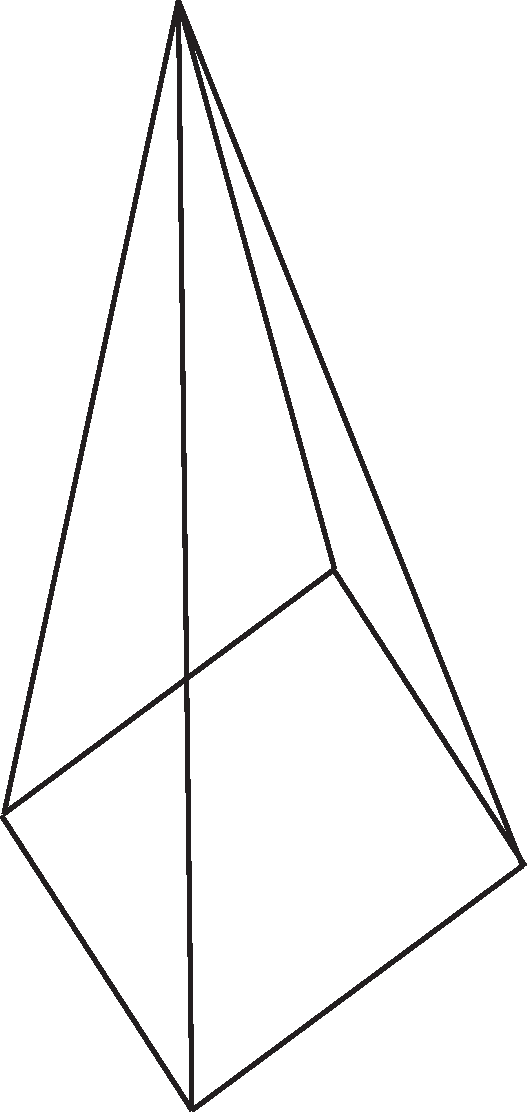
\includegraphics[width=0.18\textwidth]{images/LH37,4_49r-4.pdf}
%%\end{minipage}
%%\hspace*{-10mm}
%%\begin{minipage}[t]{0.33\textwidth}
%%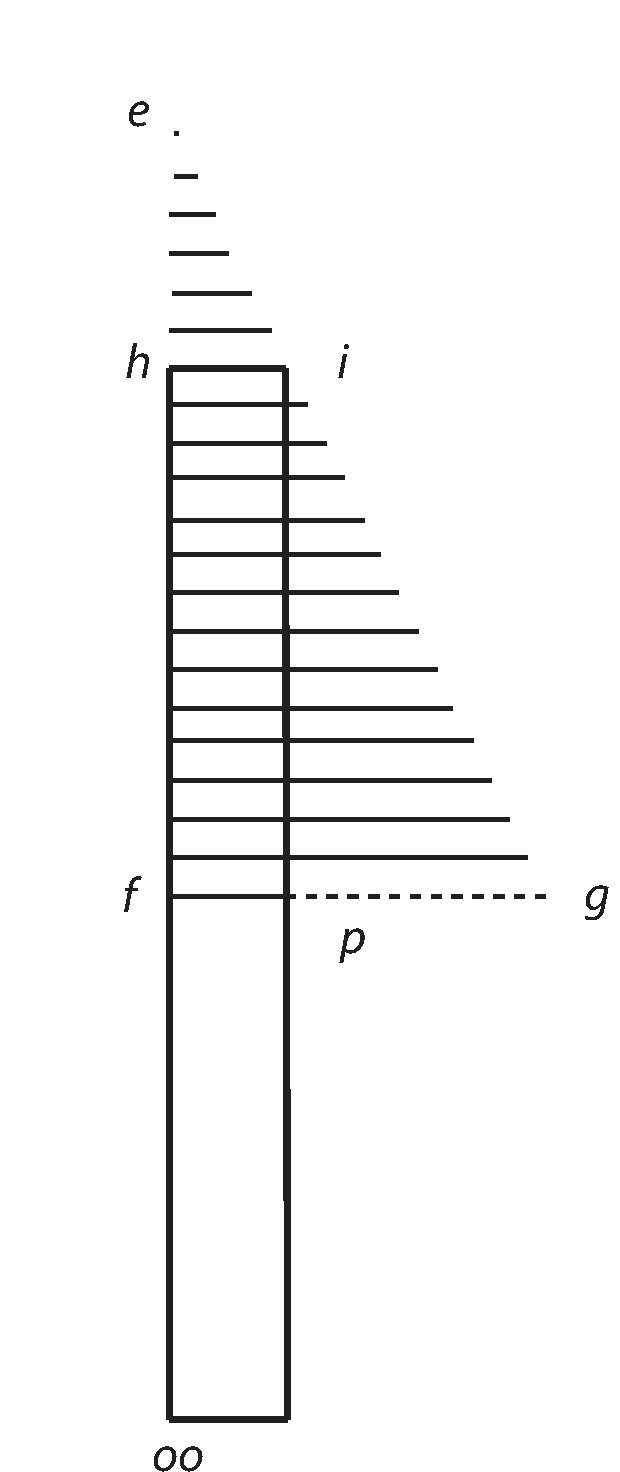
\includegraphics[width=0.6\textwidth]{images/LH37,4_49r-2.pdf}\\
%%\end{minipage}
%%\hspace*{-1mm}  [\textit{Fig. 2}]\hspace*{44mm}  [\textit{Fig. 3}]\hspace*{38mm}  [\textit{Fig. 4}]
%%\pend
%%\vspace*{2em}% PR: Rein provisorisch !!!
%%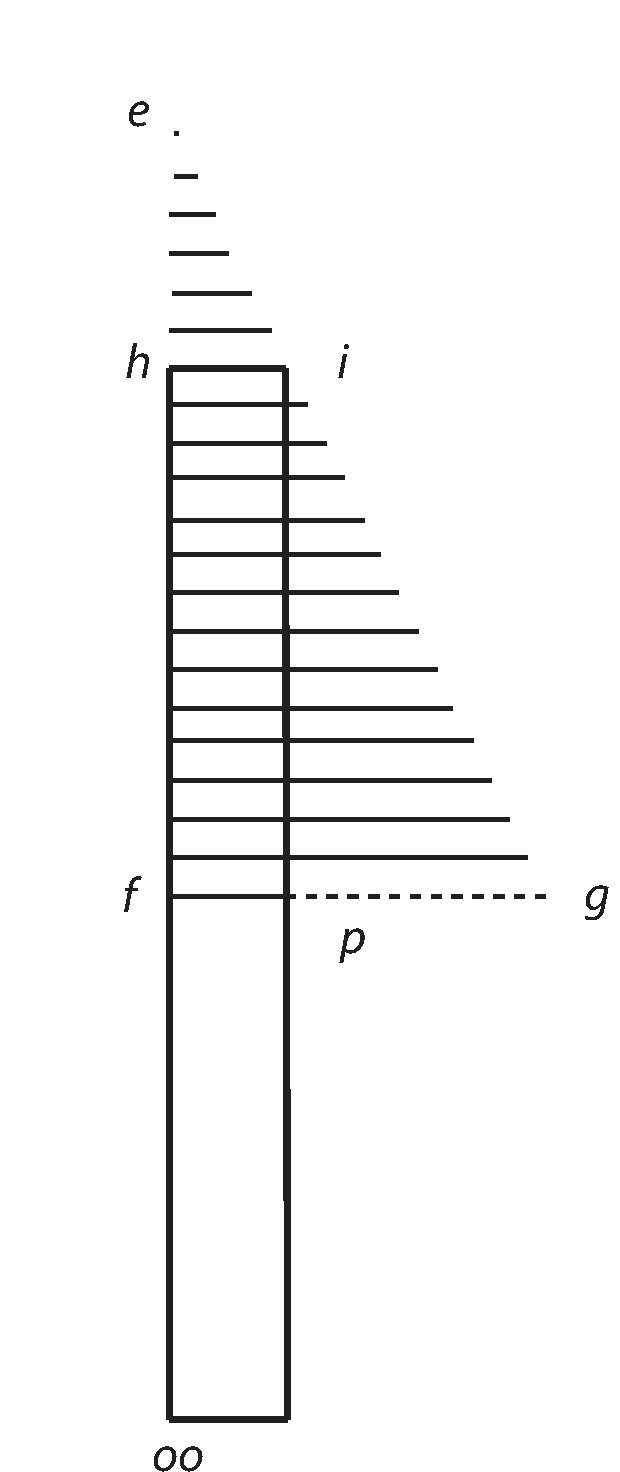
\includegraphics[width=0.3\textwidth]{images/LH37,4_49r-2.pdf}
%%\pstart%
%\hspace*{7.5mm}His positis 
quantitatem ponderis\protect\index{Sachverzeichnis}{pondus} $n$ ita investigo, cum eo ad $ab$ adjecto, et ex puncto $b$ suspenso potentia $ab$ aequetur potentiae $ca$ ergo $mc$ aequabitur ipsi $n$.
Hujus $mc$ potentia est ad potentiam $ma$ vel $ab$ ut Trapezium seu Triangulum truncatum $hifg$ ad Triangulum $ehi$ hinc si intelligatur Trabem horizonti parallelam $mc$ suspendi perpendiculariter ex $m$ \edtext{ut $mmcc$}{\lemma{ut $mmcc$}\Bfootnote{\textit{erg. L}}} manifestum est ejus potentiam in situ perpendiculari, ad potentiam in situ parallelo, esse ut rectangulum $fhi$ ad Trapezium $higf$ et ideo rectangulum $mmcc$ vel $hif$ produci debere longius illud \edtext{usque}{\lemma{usque}\Bfootnote{\textit{erg. L}}} in $o$ hoc in $oo$ ut Trapezio\protect\index{Sachverzeichnis}{trapezium} aequentur.\\
%\pend
%\pstart
\hspace*{7.5mm}Hinc patet rationem $hi$ ad $eh$ seu $ck$ spissitudinis cylindri, ad $ab$ brachium \edtext{minus determinare}{\lemma{minus}\Bfootnote{\textit{(1)}\ sive punctu \textit{(2)}\ a \textit{(3)}\ determinare \textit{L}}} nobis Triangulum $efg$ ita enim est $fg$ ad $ef$ ut $hi$ ad $eh$ quodsi ergo $fg$ intelligatur triplum $hi$ exempli causa; Triangulum $ipg$ erit aequale rectangulo $hif$ et rectangulum $hif$ duplicatum seu $hioo$ \edtext{vel $mmccoo$}{\lemma{vel $mmccoo$}\Bfootnote{\textit{erg. L}}}, aequale erit Trapezio $hifg$ ergo $mmo$ suspensum ex $m$ perpendiculariter tantum valet quantum $mc$ \edtext{suspensum paralleliter}{\lemma{suspensum}\Bfootnote{\textit{(1)}\ perpendiculariter \textit{(2)}\ paralleliter. \textit{L}}}.
Quodsi ergo $mmo$ sit duplum $mc$ et $mc$ librarum 3 erit  $mmo$, sive (si in unum colligatur) pondus\protect\index{Sachverzeichnis}{pondus} $n$ librarum 6.%
\edtext{}{\lemma{}\Afootnote{\textit{Am Rand, quer:}
\newline
Non possunt comparari pondus in vecte cum pondere extra vectem.\textsuperscript{[a]}
Nam si $m$ incipere intelligatur ab $a$[,] $mq$ vel $ck$ erit punctum, nec ejus ratio erit dabilis ad $am$.
Ergo nec inveniri poterit $co$.%
% PR: Marginalienapparat:
\vspace*{2mm}% 
\newline%
\footnotesize%
\textsuperscript{[a]}\ \textit{(1)}\ Nota evenire non potest, ut trabs immediate attin\ \textit{(2)}\ Non possunt [...] extra vectem. \textit{L}\vspace{-4mm}%
}}
[49~v\textsuperscript{o}]
\pend
\count\Afootins=1200
\count\Bfootins=1200
\count\Cfootins=1200
\pstart%
Idem breviori calculo apparet ex centro gravitatis\protect\index{Sachverzeichnis}{gravitas}, quod ita facile ostendo.
Opus est 16 contra 4 si utrumque ex centro gravitatis\protect\index{Sachverzeichnis}{gravitas} seu medio suae Trabis suspendatur,
duplicetur potentia ejus quod ex trabe minore pendet,
ut pendeat non ex medio \edtext{sed ex extremo}{\lemma{sed ex}\Bfootnote{\textit{(1)}\ centro \textit{(2)}\ extremo \textit{L}}}
eo ipso  
\edtext{sufficit dimidiari}{\lemma{sufficit}\Bfootnote{\textit{(1)}\ duplicari \textit{(2)}\ dimidiari \textit{L}}}
pondus\protect\index{Sachverzeichnis}{pondus} seu pro 16 adhiberi 8. Ergo 7
\edtext{librae}{\lemma{librae}\Bfootnote{\textit{erg. L}}}
suspensae ex $b$ faciant brachium $ab$ aequiponderare brachio $ca$.
\pend
\vspace{2em}% PR: Rein provisorisch !!!
\pstart%
\begin{center}%
% \begin{wrapfigure}{l}{0.4\textwidth}
\hspace{20mm}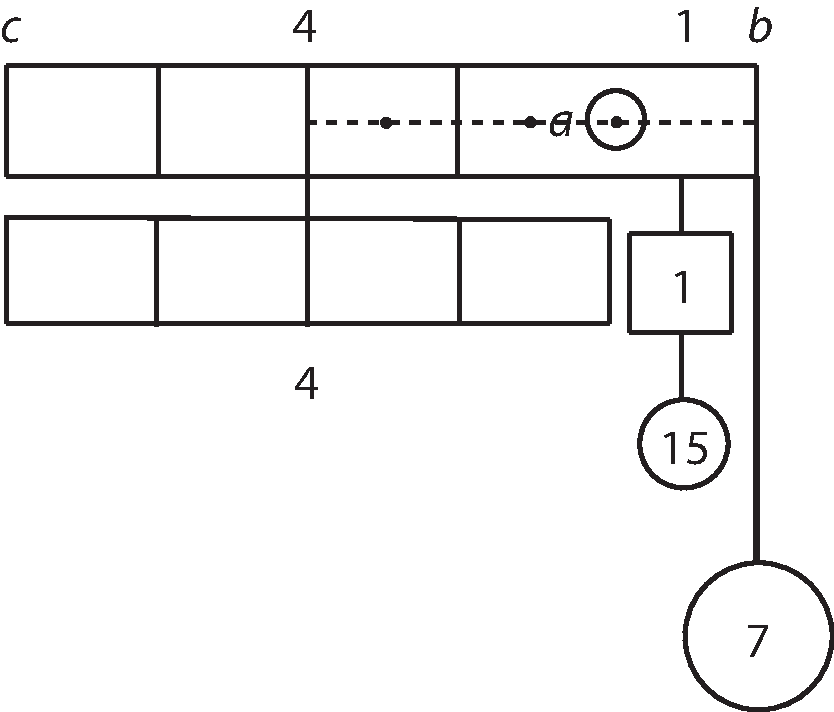
\includegraphics[width=0.45\textwidth]{images/LH37,4_49v-1.pdf}\
\vspace{0.5em}% PR: Rein provisorisch !!!
\newline%
[\textit{Fig. 5}]  
% \end{wrapfigure}
\end{center}
\pend
\vspace{2em}
%\newpage
\pstart
Sed \setline{8}quid si non Trabs sed prisma Triangulare supponatur esse $ac$.
\pend
%\vspace{2em}
\pstart
\noindent\centering
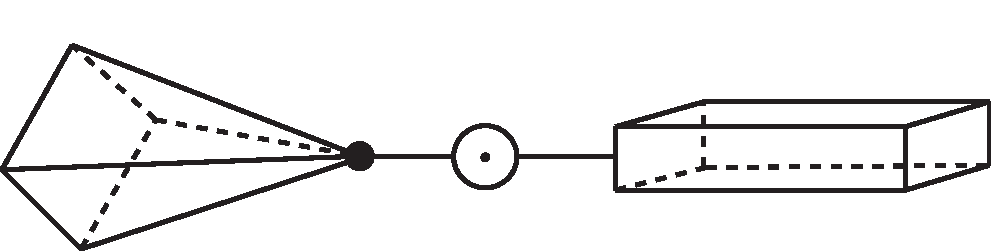
\includegraphics[trim = 0mm -3mm 0mm 0mm, clip, width=0.82\textwidth]{images/LH37,4_49v-2.pdf}\\
\noindent \centering [\textit{Fig. 6}]
\pend
\vspace{4em}
\pstart
\noindent\centering
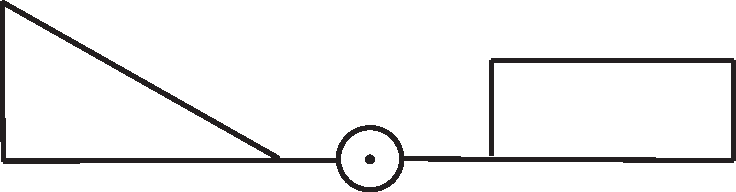
\includegraphics[trim = 0mm -3mm 0mm 0mm, clip, width=0.62\textwidth]{images/LH37,4_49v-3.pdf}\\
\setline{1}\noindent \centering [\textit{Fig. 7}]
\pend
\vspace{4em}
\pstart
\noindent\centering
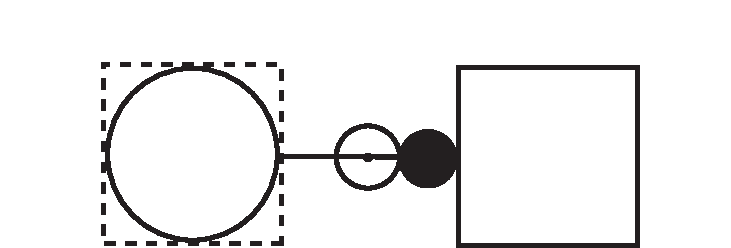
\includegraphics[trim = 0mm -3mm 0mm 0mm, clip, width=0.6\textwidth]{images/LH37,4_49v-4.pdf}\\
\noindent \centering [\textit{Fig. 8}]
\pend 
\count\Afootins=1500
\count\Bfootins=1500
\count\Cfootins=1500
%
%\begin{wrapfigure}{l}{0.4\textwidth}
%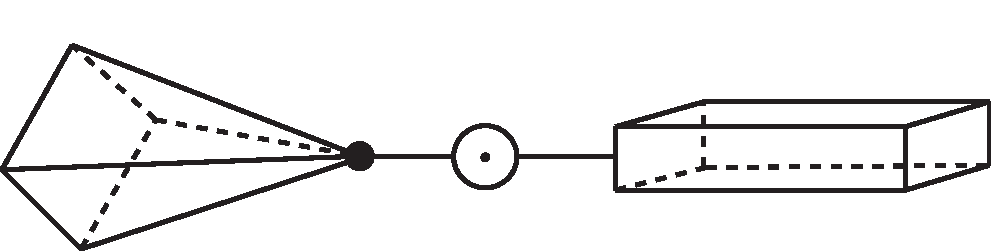
\includegraphics[width=0.4\textwidth]{images/LH37,4_49v-2.pdf}\\
%\noindent \centering [\textit{[Fig. 6]}]\\
%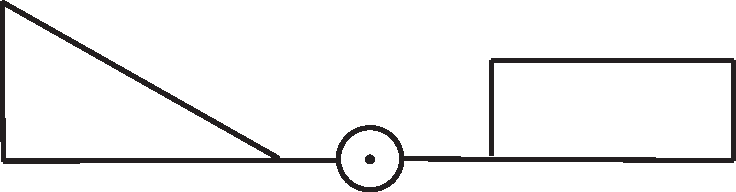
\includegraphics[width=0.4\textwidth]{images/LH37,4_49v-3.pdf}\\
%\noindent \centering [\textit{[Fig. 7]}] \\
% 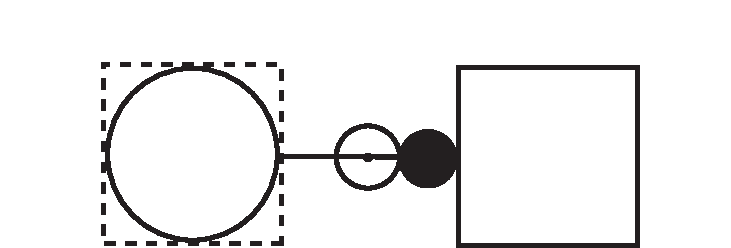
\includegraphics[width=0.4\textwidth]{images/LH37,4_49v-4.pdf}\\
%\noindent \centering [\textit{[Fig. 8]}] 
%\end{wrapfigure}
%